\begin{figure*}[p]
\centering
\input{figures/hp-grid-marks}
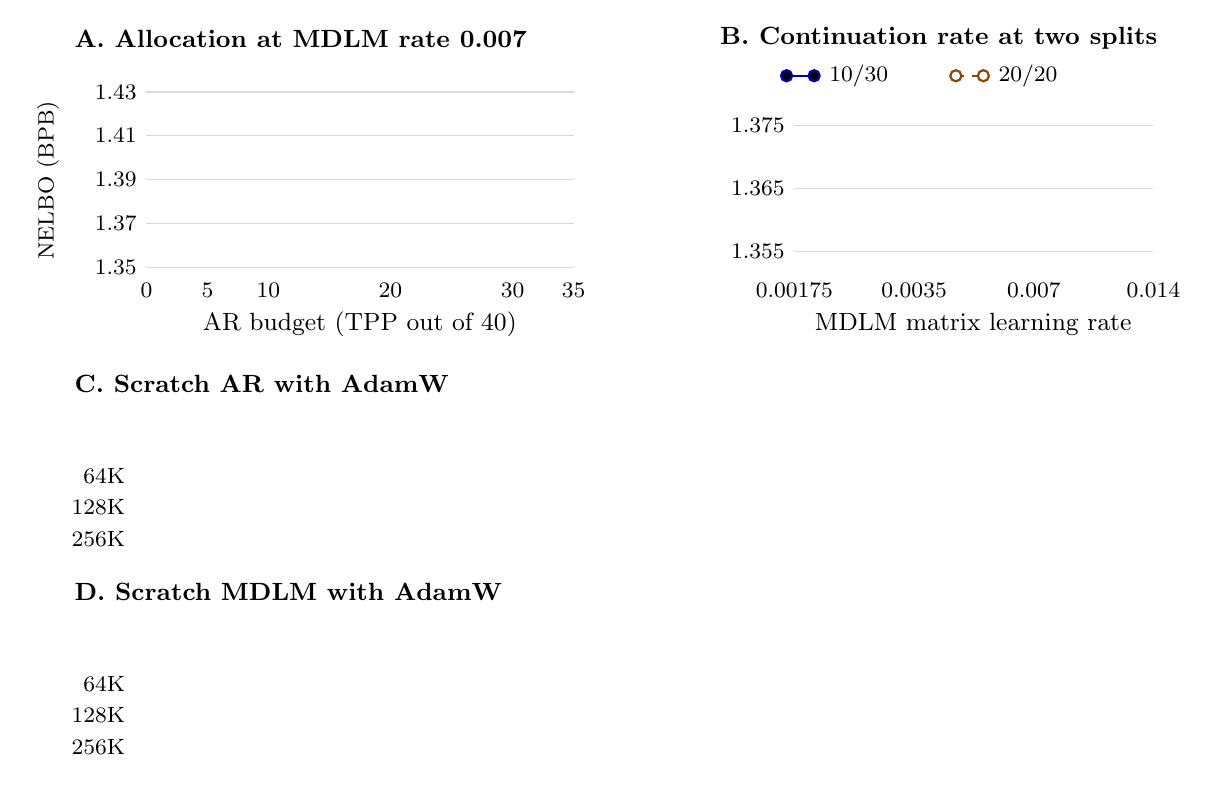
\begin{tikzpicture}[font=\small,
  allocation/.style={thick,draw=teal!70!black,mark=*},
  quarter/.style={thick,draw=blue!70!black,mark=*},
  half/.style={thick,dashed,draw=orange!55!black,mark=*,mark options={solid,fill=white,draw=orange!55!black}},
  heading/.style={anchor=west,font=\small\bfseries,inner sep=0pt},
  tick/.style={font=\footnotesize}]
\node[heading] at (0,3.85) {A. Allocation at MDLM rate 0.007};
\node[rotate=90,tick] at (-0.33,2.05) {NELBO (BPB)};
\node[heading] at (8.2,3.85) {B. Continuation rate at two splits};
\begin{scope}[shift={(0.92,0.95)},x=0.155cm,y=27.8cm]
  \pgftransformshift{\pgfpointxy{0}{-1.35}}
  \foreach \y in {1.35,1.37,1.39,1.41,1.43}{
    \draw[black!15] (0,\y)--(35,\y);
    \node[left,tick] at (0,\y) {\y};}
  \allocationcurve
  \foreach \x in {0,5,10,20,30,35}{\node[below,tick] at (\x,1.347) {\x};}
\end{scope}
\node at (3.63,0.22) {AR budget (TPP out of 40)};
\begin{scope}[shift={(9.15,0.95)},x=1.52cm,y=80cm]
  \pgftransformshift{\pgfpointxy{0}{-1.3525}}
  \foreach \y in {1.355,1.365,1.375}{
    \draw[black!15] (0,\y)--(3,\y);
    \node[left,tick] at (0,\y) {\y};}
  \quartercurve
  \halfcurve
  \foreach \x/\lr in {0/0.00175,1/0.0035,2/0.007,3/0.014}{
    \node[below,tick] at (\x,1.3515) {\lr};}
\end{scope}
\node at (11.42,0.22) {MDLM matrix learning rate};
\draw[quarter] plot coordinates {(9.05,3.38)(9.40,3.38)};
\node[right,tick] at (9.47,3.38) {10/30};
\draw[half] plot coordinates {(11.2,3.38)(11.55,3.38)};
\node[right,tick] at (11.62,3.38) {20/20};

\definecolor{scoreblue}{RGB}{108,179,192}
\def\budgettitle#1#2{\node[font=\footnotesize\bfseries] at ({3.24*#1+1},1.75) {#2 TPP};}
\def\ratelabel#1#2{\node[tick] at (#1,0.93) {#2};}
\def\scorecell#1#2#3#4{%
  \fill[scoreblue!#4] ({#1-.49},{#2-.48}) rectangle ({#1+.49},{#2+.48});
  \node[tick] at (#1,#2) {#3};}
\def\gridpanel#1#2#3{%
  \node[heading] at (0,{#1+1.17}) {#2};
  \begin{scope}[shift={(1.32,#1)},x=1.07cm,y=.40cm]
    \foreach \y/\batch in {0/64K,-1/128K,-2/256K}{
      \node[left,tick] at (-.51,\y) {\batch};}
    #3
  \end{scope}}
\gridpanel{-1.70}{C. Scratch AR with AdamW}{\argrid}
\gridpanel{-4.34}{D. Scratch MDLM with AdamW}{\mdlmgrid}
\end{tikzpicture}
\caption{\textbf{Training grids at 20M parameters.} A and B show document-start NELBO in bits per byte (BPB) for the Muon study. A varies the AR share at fixed total budget. B varies the MDLM rate for two AR/MDLM splits. C and D show the separate scratch AdamW grids. Rows give tokens per update (K means 1,024). Within each budget, columns give peak learning rate in units of $10^{-3}$. Cells show validation BPB, with darker shading for lower loss within each panel. C measures causal log loss and D measures masked reconstruction. Each panel uses one training seed. The companion tables give exact rates and scores for all tested cells.}
\label{fig:hp-grids}
\end{figure*}
